\documentclass{article}

\usepackage{arxiv}
\usepackage[utf8]{inputenc}
\usepackage[T1]{fontenc}
\usepackage{hyperref}
\usepackage{url}
\usepackage{booktabs}
\usepackage{amsfonts}
\usepackage{amsmath}
\usepackage{amssymb}
\usepackage{amsthm}
\usepackage{nicefrac}
\usepackage{microtype}
\usepackage{graphicx}
\usepackage[numbers]{natbib}
\usepackage{doi}
\usepackage{placeins}

\newtheorem{definition}{Definition}
\newtheorem{proposition}{Proposition}
\newtheorem{theorem}{Theorem}
\newtheorem{corollary}{Corollary}
\newtheorem*{remark}{Remark}

\newcommand{\vect}[1]{\mathbf{#1}}
\newcommand{\mat}[1]{\mathbf{#1}}
\newcommand{\R}{\mathbb{R}}
\newcommand{\Sph}{\mathbb{S}}

\newcommand\figref{Figure~\ref}
\renewcommand\eqref{Equation~\ref}
\newcommand\tabref{Table~\ref}
\newcommand*{\secref}[1]{\hyperref[{#1}]{\S\ref*{#1}}}

\title{Flat Gaussian Embedding Spaces for Change Detection:\\
Geometric Foundations and Capacity Analysis}

\author{%
    \href{https://orcid.org/0000-0002-7227-4946}{
\includegraphics[scale=0.06]{orcid.pdf}\hspace{1mm}Shreeyam Kacker} \\
    Department of Aeronautics and Astronautics \\
    MIT \\
    \texttt{shreeyam@mit.edu}
}

\renewcommand{\headeright}{}
\renewcommand{\undertitle}{}
\renewcommand{\shorttitle}{Flat Gaussian Embeddings for Change Detection}

\hypersetup{%
    pdftitle={Flat Gaussian Embedding Spaces for Change Detection},
    pdfsubject={cs.CV, cs.LG},
    pdfauthor={Shreeyam Kacker},
    pdfkeywords={change detection, self-supervised learning, embedding geometry, Sidon sets}
}

\begin{document}
\maketitle

\begin{abstract}
Change detection via embedding differencing---computing $\vect{\delta} = \vect{z}_{t_2} - \vect{z}_{t_1}$ between learned representations---is appealing for its simplicity, but is only valid on a geometry that makes such differences meaningful. We show that the hypersphere, the implicit geometry of DINO-family encoders \citep{caron2021emerging, oquab2023dinov2, wu2025simdino}, is not such a geometry: geodesic differences are not composable, ambient Euclidean differences are not semantically consistent, and concatenation-based alternatives discard geometric structure entirely. These are not empirical shortcomings but topological obstructions inherent to any positively curved embedding manifold. A flat embedding space---one where representations live in $\R^d$ without normalization---resolves all three problems simultaneously and makes Euclidean subtraction a composable, transitive change operator. Regularizing this space toward an isotropic Gaussian further ensures that change magnitudes are calibrated across the embedding space. We then quantify the cost of flatness: using a Poisson approximation \citep{barbour1992poisson} to a continuous analog of the classical Sidon set problem \citep{erdos1941problem, halberstam1983sequences}, we derive closed-form expressions for the capacity of a flat embedding space---the number of points at which the probability of a collision among pairwise differences reaches $1/2$---under isotropic Gaussian, uniform ball, and uniform sphere distributions, and verify them with Monte Carlo simulation.
\end{abstract}

\noindent\textbf{Keywords:} change detection, embedding geometry, Sidon sets, self-supervised learning

% ==============================================================
\section{Introduction}
\label{sec:introduction}

Change detection from satellite imagery is often cast as a comparison between learned features $\vect{z}_{t_1}$ and $\vect{z}_{t_2}$ of the same scene at two times \citep{daudt2018fullycnn, chen2020dasnet, bovolo2007cva}. A natural strategy is to represent the change by the feature difference $\vect{\delta} = \vect{z}_{t_2} - \vect{z}_{t_1}$: it is parameter-free, composable, and inherits whatever structure the feature space provides. For this to be principled, however, the feature space must admit a well-defined notion of ``difference.''

Modern self-supervised encoders---DINO \citep{caron2021emerging}, DINOv2 \citep{oquab2023dinov2}, and their descendants---$\ell_2$-normalize their outputs, placing embeddings on the unit hypersphere $\Sph^{d-1}$ rather than in $\R^d$. On a curved manifold, subtraction is no longer well-defined: the intrinsic analog (the logarithmic map) produces vectors in different tangent spaces that cannot be composed without path-dependent parallel transport, and the extrinsic shortcut of subtracting ambient coordinates breaks semantic consistency. These are geometric obstructions, not empirical ones---no amount of training data or architectural tuning resolves them.

This paper makes two contributions:
\begin{enumerate}
    \item \textbf{Curvature sets a hard error floor on the hypersphere.} We formalize a change vector as a group-valued difference operator generalizing subtraction, and prove that any approximate change-vector operator on $\Sph^{d-1}$ has a composability error that scales with the spherical excess of the points involved (Proposition~\ref{prop:composability_floor}): the error grows as embeddings spread across the sphere and cannot be trained away. A stronger topological impossibility holds for $d \notin \{1,2,4\}$ but is cosmetic next to the curvature floor. Ambient differencing fails semantic consistency (Proposition~\ref{prop:ambient_bad}) and concatenation discards geometry entirely. Flatness removes all three obstructions, and isotropy calibrates magnitudes (Propositions~\ref{prop:flat_sufficient}, \ref{prop:isotropy_calibration}).
    \item \textbf{Capacity of flat embedding spaces.} We quantify the cost: how many points can a flat space host before pairwise differences collide? Framing this as a continuous Sidon set problem, we derive closed-form expressions for collision probability and capacity under Gaussian, ball, and sphere distributions and verify them empirically (\secref{sec:capacity}, \secref{sec:empirical}).
\end{enumerate}

% ==============================================================
% \section{Related Work}
% \label{sec:related}
%
% TODO: Change detection methods (feature differencing, concatenation,
% correlation-based), self-supervised representation learning (DINO,
% MAE, contrastive methods), geometry of representation spaces
% (hyperbolic embeddings, normalization effects), Sidon sets and
% additive combinatorics.

% ==============================================================
\section{Analysis}
\label{sec:analysis}

Let $f : \mathcal{X} \to \R^d$ be a learned encoder mapping inputs to a $d$-dimensional embedding space. In methods such as DINO \citep{caron2021emerging}, the output is $\ell_2$-normalized so that embeddings lie on $\Sph^{d-1} = \{ \vect{z} \in \R^d : \|\vect{z}\| = 1 \}$. We consider two observations $x_1, x_2 \in \mathcal{X}$ of the same scene at different times, producing embeddings $\vect{z}_1 = f(x_1)$ and $\vect{z}_2 = f(x_2)$, and ask: under what conditions is their difference a meaningful representation of the change between the two scenes?

\subsection{Definitions}

Let $\mathcal{Z} = f(\mathcal{X}) \subseteq \R^d$ denote the image of the encoder, $(G, \cdot)$ a group with identity $e$, and $\mathcal{C} : \mathcal{X} \to \mathcal{Y}$ a labeling that assigns each input a semantic class.

\begin{definition}[Change Vector]
\label{def:change_vector}
A \emph{change vector} is a map $\Delta : \mathcal{Z} \times \mathcal{Z} \to G$ satisfying:
\begin{enumerate}
    \item[(i)] \textbf{Invertibility:} for each $\vect{z}_1 \in \mathcal{Z}$ and $g \in G$, there is a unique $\vect{z}_2 \in \mathcal{Z}$ with $\Delta(\vect{z}_1, \vect{z}_2) = g$.
    \item[(ii)] \textbf{Composability:} for any $\vect{a}, \vect{b}, \vect{c} \in \mathcal{Z}$,
    \[
        \Delta(\vect{a}, \vect{b}) \cdot \Delta(\vect{b}, \vect{c}) = \Delta(\vect{a}, \vect{c}).
    \]
\end{enumerate}
\end{definition}

\noindent The axioms force $\Delta(\vect{a}, \vect{a}) = e$ and $\Delta(\vect{b}, \vect{a}) = \Delta(\vect{a}, \vect{b})^{-1}$, and make $(\mathcal{Z}, G, \Delta)$ a principal homogeneous space (torsor): $G$ acts freely and transitively on $\mathcal{Z}$, and $\Delta$ recovers the unique group element carrying one point to another. Concretely, under any identification $\mathcal{Z} \cong G$ we have $\Delta(\vect{z}_1, \vect{z}_2) = \vect{z}_1^{-1} \vect{z}_2$. In the Euclidean case $G = (\R^d, +)$ the inverse is negation, and $\Delta$ reduces to ordinary subtraction $\vect{z}_2 - \vect{z}_1$---the abelian group hides the need for a left--right distinction, but the structure is what makes the subtraction \emph{mean} anything.

\begin{remark}[Path-independence is automatic]
\label{rem:path_independence}
Defining $\Delta$ as a function $\mathcal{Z} \times \mathcal{Z} \to G$ forces \emph{path-independence}: the change vector depends only on the endpoints, not on any curve between them. On $\R^d$ this is trivial. On $\Sph^{d-1}$ the intrinsic analog---the logarithmic map---is not path-independent once tangent vectors from different base points are compared, foreshadowing Proposition~\ref{prop:composability_floor}.
\end{remark}

\begin{definition}[Semantic Consistency]
\label{def:semantic_consistency}
A change representation $\Delta$ is \emph{semantically consistent} with respect to $\mathcal{C}$ if, for all $x_1, x_1', x_2, x_2' \in \mathcal{X}$ with $\mathcal{C}(x_1) = \mathcal{C}(x_1')$ and $\mathcal{C}(x_2) = \mathcal{C}(x_2')$,
\[
    \Delta\!\bigl(f(x_1),\, f(x_2)\bigr) = \Delta\!\bigl(f(x_1'),\, f(x_2')\bigr).
\]
\end{definition}

\noindent Semantic consistency is an idealization: it corresponds to the zero intra-class variance limit. We adopt it deliberately---if a change representation fails here, no approximate version can succeed.

\paragraph{Euclidean subtraction is a change vector.} In $\R^d$ with $G = (\R^d, +)$, $\Delta(\vect{z}_1, \vect{z}_2) = \vect{z}_2 - \vect{z}_1$ satisfies the axioms trivially, and semantic consistency holds whenever $f$ maps each class to a single point $\vect{c}_y$, since $\Delta(f(x_1), f(x_2)) = \vect{c}_{\mathcal{C}(x_2)} - \vect{c}_{\mathcal{C}(x_1)}$ depends only on the classes. The question is whether any analogous structure survives on a curved manifold; it does not.

\paragraph{The hypersphere has a curvature-driven error floor.}
\label{sec:sphere_failures}

In ML we rarely require \emph{exact} composability; the relevant question is how much error an approximate change-vector operator incurs. On the hypersphere, that error has a hard floor set by curvature.

\begin{proposition}[Curvature-driven composability floor]
\label{prop:composability_floor}
Let $\Delta : \Sph^{d-1} \times \Sph^{d-1} \to G$ be any continuous approximate change-vector operator. The composability residual
\[
    r(\vect{a}, \vect{b}, \vect{c}) = d_G\!\bigl(\Delta(\vect{a}, \vect{b}) \cdot \Delta(\vect{b}, \vect{c}),\; \Delta(\vect{a}, \vect{c})\bigr)
\]
cannot vanish uniformly. For $\Delta$ built from the logarithmic map, $r$ is bounded below by the spherical excess of the geodesic triangle $(\vect{a}, \vect{b}, \vect{c})$---which by the Ambrose--Singer holonomy theorem \citep{ambrose1953theorem} scales as $\Theta(\mathrm{Area})$ and grows with the spread of the points on the sphere.
\end{proposition}

\noindent The mechanism is parallel transport: the logarithmic map
\begin{equation}
    \log_{\vect{z}_1}(\vect{z}_2) = \frac{\theta}{\sin\theta}\left(\vect{z}_2 - \cos\theta \cdot \vect{z}_1\right), \qquad \theta = \arccos\langle \vect{z}_1, \vect{z}_2 \rangle,
\end{equation}
lives in a base-point-dependent tangent space, and transporting between tangent spaces on a positively curved manifold accumulates a rotation proportional to the enclosed area. Since DINO embeddings are typically spread across the sphere, this error is not a small correction---it is the dominant failure mode.

An even stronger statement holds: no operator on $\Sph^{d-1}$ can achieve composability \emph{exactly}, regardless of construction.\footnote{A change vector makes $(\Sph^{d-1}, G, \Delta)$ a $G$-torsor, so $G \cong \Sph^{d-1}$ as a smooth manifold. By Adams' theorem the only parallelizable spheres are $\Sph^0, \Sph^1, \Sph^3, \Sph^7$; of these, $\Sph^7$ admits no group structure (octonion multiplication is non-associative). So for $d \notin \{1, 2, 4\}$ no exact change vector exists. ML-wise this refinement is cosmetic---Proposition~\ref{prop:composability_floor} already shows any approximate operator has an area-scaling error floor.} In ML terms: even the best possible approximation cannot do better than this curvature-dependent error.

\paragraph{Ambient subtraction: not semantically consistent.}

\begin{proposition}
\label{prop:ambient_bad}
For $\vect{z}_1, \vect{z}_2 \in \Sph^{d-1}$, the ambient difference $\vect{z}_2 - \vect{z}_1$ is not semantically consistent. Its magnitude $\|\vect{b} - \vect{a}\|^2 = 2 - 2\langle \vect{a}, \vect{b}\rangle$ varies with the inner product across class instances, and for any rotation $R$ mapping $(\vect{a}, \vect{b}) \to (\vect{a}', \vect{b}')$, $\vect{b}' - \vect{a}' = R(\vect{b} - \vect{a})$---the change vector rotates with absolute position.
\end{proposition}

\paragraph{Pair concatenation: not a geometric object.} A third alternative discards differencing and feeds $[\vect{z}_1; \vect{z}_2] \in \R^{2d}$ to a learned head. No group operation $\cdot$ satisfies $[\vect{a}; \vect{b}] \cdot [\vect{b}; \vect{c}] = [\vect{a}; \vect{c}]$, so the result violates Definition~\ref{def:change_vector}. The learned head must observe every pair type during training, and the $2d$-dimensional output carries no geometric meaning: it is a black-box pairwise classifier, not a representation.\label{rem:concatenation}

\subsection{Flatness and Isotropy}
\label{sec:flat_sufficient}

The three failure modes above---intrinsic non-composability, extrinsic semantic inconsistency, and the non-geometry of concatenation---share a common root: curvature. Removing it resolves all three simultaneously.

\begin{proposition}[Flatness suffices for well-defined change vectors]
\label{prop:flat_sufficient}
Let $f : \mathcal{X} \to \R^d$ be an encoder whose image $\mathcal{Z} = f(\mathcal{X})$ lies in $\R^d$ without normalization to a curved submanifold. Then $\Delta(\vect{z}_1, \vect{z}_2) = \vect{z}_2 - \vect{z}_1$ satisfies Definition~\ref{def:change_vector}, and if $f$ maps each semantic class to a compact cluster with center $\vect{c}_y$, then $\Delta$ is approximately semantically consistent: $\|\Delta(f(x_1), f(x_2)) - (\vect{c}_{\mathcal{C}(x_2)} - \vect{c}_{\mathcal{C}(x_1)})\| \le \mathrm{diam}(\mathcal{C}(x_1)) + \mathrm{diam}(\mathcal{C}(x_2))$, where $\mathrm{diam}(y)$ is the diameter of the cluster for class $y$.
\end{proposition}

\begin{proof}
The change vector axioms hold by the trivial verification in \secref{sec:analysis}: $\R^d$ is flat, parallel transport is the identity, and vector addition is globally defined. For semantic consistency, write $f(x_i) = \vect{c}_{\mathcal{C}(x_i)} + \vect{\epsilon}_i$ with $\|\vect{\epsilon}_i\| \le \mathrm{diam}(\mathcal{C}(x_i))$. Then
\[
    \Delta(f(x_1), f(x_2)) = (\vect{c}_{\mathcal{C}(x_2)} - \vect{c}_{\mathcal{C}(x_1)}) + (\vect{\epsilon}_2 - \vect{\epsilon}_1),
\]
and $\|\vect{\epsilon}_2 - \vect{\epsilon}_1\| \le \mathrm{diam}(\mathcal{C}(x_1)) + \mathrm{diam}(\mathcal{C}(x_2))$ by the triangle inequality. In the zero intra-class variance limit ($\mathrm{diam} \to 0$), exact semantic consistency is recovered.
\end{proof}

Flatness alone makes differencing well-defined, but says nothing about the \emph{scale} of change vectors across the embedding space. A flat space with highly anisotropic features---variance concentrated along a few dimensions---would produce change vectors whose magnitude depends on direction rather than semantic content. Isotropy resolves this.

\begin{proposition}[Isotropy calibrates change magnitude]
\label{prop:isotropy_calibration}
Let $\vect{z} \sim \mu$ with $\mathrm{Cov}[\vect{z}] = \sigma^2 \mat{I}_d$. For any two independent draws $\vect{z}_1, \vect{z}_2 \sim \mu$, the expected squared change magnitude satisfies
\[
    \mathbb{E}\!\left[\|\vect{z}_2 - \vect{z}_1\|^2\right] = 2d\sigma^2,
\]
independent of the positions $\vect{z}_1, \vect{z}_2$. All dimensions contribute equally to $\|\Delta\|$, and $\sigma$ is a per-dimension noise floor: a change of magnitude $\sigma$ in any single dimension contributes the same increment to $\|\Delta\|$.
\end{proposition}

\noindent This is immediate from $\mathrm{Cov}[\vect{z}_2 - \vect{z}_1] = 2\sigma^2 \mat{I}_d$ and $\mathbb{E}\|\vect{x}\|^2 = \mathrm{tr}(\mathrm{Cov}[\vect{x}])$.

\begin{remark}
Propositions~\ref{prop:flat_sufficient} and \ref{prop:isotropy_calibration} together motivate a specific embedding strategy: learn features in $\R^d$ (no $\ell_2$-normalization) and regularize toward $\mathbb{E}[f(x)] \approx \vect{0}$, $\mathrm{Cov}[f(x)] \approx \mat{I}_d$---i.e., an approximately isotropic Gaussian embedding distribution. Several existing objectives realize approximations to this prescription: the variance and covariance terms of VICReg \citep{bardes2022vicreg}, the redundancy-reduction loss of Barlow Twins \citep{zbontar2021barlow}, the maximal coding rate reduction objective \citep{yu2020mcr2, ma2007segmentation}, and the Gaussianity regularizer of SigReg \citep{schaeffer2024sigreg} all push covariances toward identity via different mechanisms. SimDINO \citep{wu2025simdino} demonstrates that a single coding-rate regularizer can replace the entire DINO sharpening-and-centering pipeline. This makes Euclidean subtraction a composable, semantically consistent, and calibrated change operator.
\end{remark}

\begin{corollary}[Approximate composability has a curvature-dependent error floor]
\label{cor:approx_floor}
Let $\Delta : \Sph^{d-1} \times \Sph^{d-1} \to G$ be any continuous map
satisfying invertibility. Then the composability residual
\[
    r(\vect{a}, \vect{b}, \vect{c})
    = d_G\!\bigl(\Delta(\vect{a}, \vect{b}) \oplus \Delta(\vect{b}, \vect{c}),\;
                  \Delta(\vect{a}, \vect{c})\bigr)
\]
cannot vanish uniformly: $\sup_{\vect{a},\vect{b},\vect{c}} r(\vect{a},
\vect{b}, \vect{c}) > 0$. If $\Delta$ is constructed from the logarithmic
map, the residual is bounded below by the spherical excess of the geodesic
triangle, which scales as $\Theta(\mathrm{Area})$ and is nonzero for every
non-degenerate triple.
\end{corollary}

% ==============================================================
\subsection{Capacity of Embedding Spaces}
\label{sec:capacity}

We now fix a flat embedding space and ask a quantitative question: how many distinct points can such a space host before pairwise differences begin to collide? A \emph{collision} occurs when two distinct ordered pairs $(i,j)$ and $(k,l)$ produce difference vectors $\vect{X}_i - \vect{X}_j$ and $\vect{X}_k - \vect{X}_l$ within $L_2$ distance $\varepsilon$ of each other. Collisions are precisely the regime in which two different transitions produce indistinguishable change vectors---the failure mode that \secref{sec:geometry} was designed to prevent. This is a continuous analog of the classical Sidon set problem from additive combinatorics \citep{erdos1941problem, halberstam1983sequences}.

\subsubsection{Poisson Approximation}

The total number of ordered pairwise differences among $N$ points is $M = \binom{N}{2}$. The number of candidate collision pairs is
\begin{equation}
    K = \binom{M}{2} \approx \frac{N^4}{8}.
\end{equation}
For a single candidate pair $(\vect{X}_i - \vect{X}_j,\; \vect{X}_k - \vect{X}_l)$ with $\{i,j\} \neq \{k,l\}$, let $\vect{Z} = \vect{X}_i - \vect{X}_j - \vect{X}_k + \vect{X}_l$. Since the $\vect{X}_i$ are i.i.d., $\vect{Z}$ is a linear combination of independent draws. For a small collision tolerance $\varepsilon$,
\begin{equation}
\label{eq:p_single}
    p \;=\; \Pr(\|\vect{Z}\|_2 \le \varepsilon)
       \;\approx\; f_{\vect{Z}}(\vect{0}) \cdot V_d(\varepsilon)
       \;=\; f_{\vect{Z}}(\vect{0}) \, \frac{\pi^{d/2}}{\Gamma(d/2 + 1)} \, \varepsilon^d,
\end{equation}
where $V_d(\varepsilon)$ is the volume of the $d$-dimensional ball of radius $\varepsilon$. Individual collision events are weakly dependent and rare, so the total collision count is well-approximated by a Poisson random variable \citep{barbour1992poisson} with mean
\begin{equation}
\label{eq:lambda}
    \lambda \;=\; K \, p \;\approx\; \frac{N^4}{8} \, f_{\vect{Z}}(\vect{0}) \, \frac{\pi^{d/2}}{\Gamma(d/2 + 1)} \, \varepsilon^d.
\end{equation}
The probability of at least one collision is
\begin{equation}
\label{eq:Pc}
    P_c \;\approx\; 1 - e^{-\lambda}.
\end{equation}
Setting $P_c = 1/2$ gives $\lambda = \ln 2$, and solving for $N$ yields the \emph{capacity}:
\begin{equation}
\label{eq:capacity}
    N^\star \;=\; \left( \frac{8 \ln 2 \cdot \Gamma(d/2 + 1)}{f_{\vect{Z}}(\vect{0}) \, \pi^{d/2} \, \varepsilon^d} \right)^{1/4}.
\end{equation}

\subsubsection{Three Canonical Distributions}

By the central limit theorem \citep{durrett2019probability}, $\vect{Z} = \vect{X}_i - \vect{X}_j - \vect{X}_k + \vect{X}_l$ approaches $\mathcal{N}(\vect{0}, 4\mat{\Sigma})$ in high dimension for any distribution with covariance $\mat{\Sigma}$, regardless of the original distribution. We evaluate $f_{\vect{Z}}(\vect{0})$ for three cases.

\paragraph{Isotropic Gaussian.}
For $\vect{X} \sim \mathcal{N}(\vect{0}, \sigma^2 \mat{I}_d)$, the CLT is exact: $\vect{Z} \sim \mathcal{N}(\vect{0}, 4 \sigma^2 \mat{I}_d)$ and $f_{\vect{Z}}(\vect{0}) = (8 \pi \sigma^2)^{-d/2}$. Substituting,
\begin{align}
    P_{c,\mathrm{normal}} &\approx 1 - \exp\!\left( -\frac{N^4}{8 \, \Gamma(d/2 + 1)} \left( \frac{\varepsilon}{\sigma \sqrt{8}} \right)^d \right), \\
    N^\star_{\mathrm{normal}} &\approx \left( 8 \ln 2 \cdot \Gamma(d/2 + 1) \right)^{1/4} \left( \frac{\sigma \sqrt{8}}{\varepsilon} \right)^{d/4}.
\end{align}

\paragraph{Uniform on the unit ball.}
For points drawn uniformly from the solid unit ball in $\R^d$, the per-axis variance is $1/(d+2)$, giving $\vect{Z} \approx \mathcal{N}(\vect{0}, \tfrac{4}{d+2} \mat{I}_d)$ and $f_{\vect{Z}}(\vect{0}) \approx \left((d+2)/(8\pi)\right)^{d/2}$:
\begin{align}
    P_{c,\mathrm{ball}} &\approx 1 - \exp\!\left( -\frac{N^4}{8 \, \Gamma(d/2 + 1)} \left( \frac{\varepsilon \sqrt{d+2}}{\sqrt{8}} \right)^d \right), \\
    N^\star_{\mathrm{ball}} &\approx \left( 8 \ln 2 \cdot \Gamma(d/2 + 1) \right)^{1/4} \left( \frac{\sqrt{8}}{\varepsilon \sqrt{d+2}} \right)^{d/4}.
\end{align}

\paragraph{Uniform on the unit sphere.}
For points uniform on $\Sph^{d-1}$, per-axis variance is $1/d$, so $\vect{Z} \approx \mathcal{N}(\vect{0}, \tfrac{4}{d} \mat{I}_d)$ and $f_{\vect{Z}}(\vect{0}) \approx (d/(8\pi))^{d/2}$:
\begin{align}
    P_{c,\mathrm{sphere}} &\approx 1 - \exp\!\left( -\frac{N^4}{8 \, \Gamma(d/2 + 1)} \left( \frac{\varepsilon \sqrt{d}}{\sqrt{8}} \right)^d \right), \\
    N^\star_{\mathrm{sphere}} &\approx \left( 8 \ln 2 \cdot \Gamma(d/2 + 1) \right)^{1/4} \left( \frac{\sqrt{8}}{\varepsilon \sqrt{d}} \right)^{d/4}.
\end{align}

The Gaussian case admits exponentially more points than the ball or sphere at the same $\varepsilon$: Gaussian support extends beyond any fixed radius, so pairwise differences are more spread out and collisions are rarer.

% ==============================================================
\section{Empirical Verification}
\label{sec:empirical}

We verify the closed-form expressions of \secref{sec:capacity} via Monte Carlo simulation for all three distributions across dimensions $d \in \{2, \dots, 10\}$. At each $(N, d, \varepsilon)$ configuration, we draw $300$ independent realizations of $N$ points, enumerate all $\binom{N}{2}$ difference vectors, and count collisions among all pairs of differences.

\paragraph{Collision probability.} \figref{fig:Pc_vs_N} shows $P_c$ as a function of $N$ for each distribution at $\varepsilon = 0.5$ across several dimensions. The Poisson approximation \eqref{eq:Pc} agrees with simulation to within sampling error for the isotropic Gaussian, and the CLT-based approximations for the ball and sphere tighten as $d$ grows---consistent with the regime in which the four-point sum concentrates on its Gaussian limit. \figref{fig:Pc_vs_eps} shows the same behaviour as $\varepsilon$ is varied at fixed $N$.

\paragraph{Poisson mean.} \figref{fig:lambda} compares $\lambda$ directly with the observed mean collision count. Agreement is strong for $d \ge 3$; the mild overestimate at $d = 2$ reflects the $N^4/8$ pair-count approximation, which does not exclude candidate pairs of differences that share an endpoint.

\paragraph{Capacity.} \figref{fig:cap_vs_d} shows theoretical capacity $N^\star$ as a function of dimension. The Gaussian grows exponentially faster than compactly supported distributions. \figref{fig:cap_verify} substitutes the predicted $N^\star$ back into the simulator: the resulting $P_c$ falls consistently below $1/2$, confirming that \eqref{eq:capacity} is a conservative lower bound on true capacity. The gap shrinks with dimension and is small in the regime ($d \gtrsim 64$) where change detection is typically deployed.

\begin{figure}[t]
    \centering
    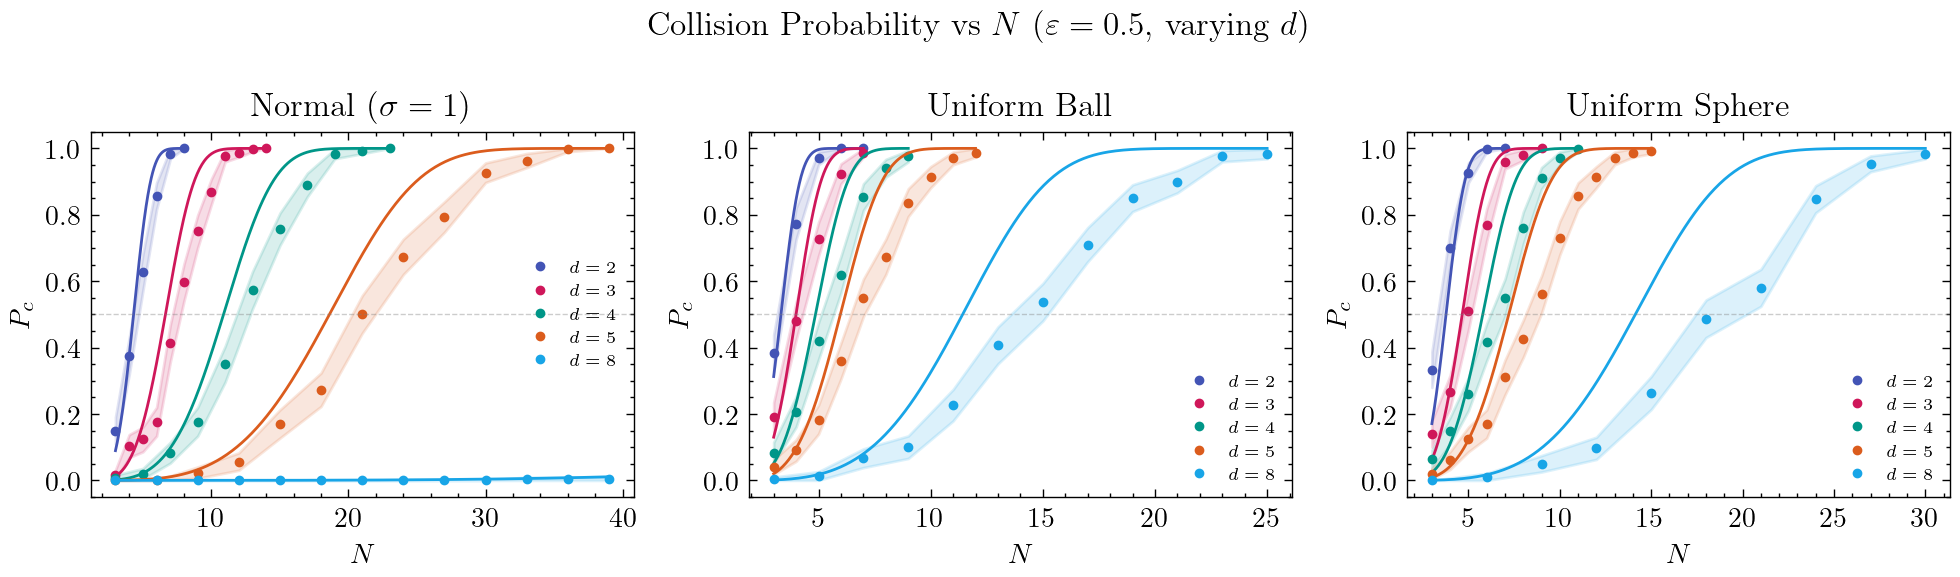
\includegraphics[width=\linewidth]{plots/Pc_vs_N.png}
    \caption{Collision probability $P_c$ as a function of $N$ at $\varepsilon = 0.5$ for $d \in \{2, 3, 4, 5, 8\}$. Solid lines: Poisson approximation \eqref{eq:Pc}. Markers: Monte Carlo estimates (300 trials) with 95\% confidence intervals.}
    \label{fig:Pc_vs_N}
\end{figure}

\begin{figure}[t]
    \centering
    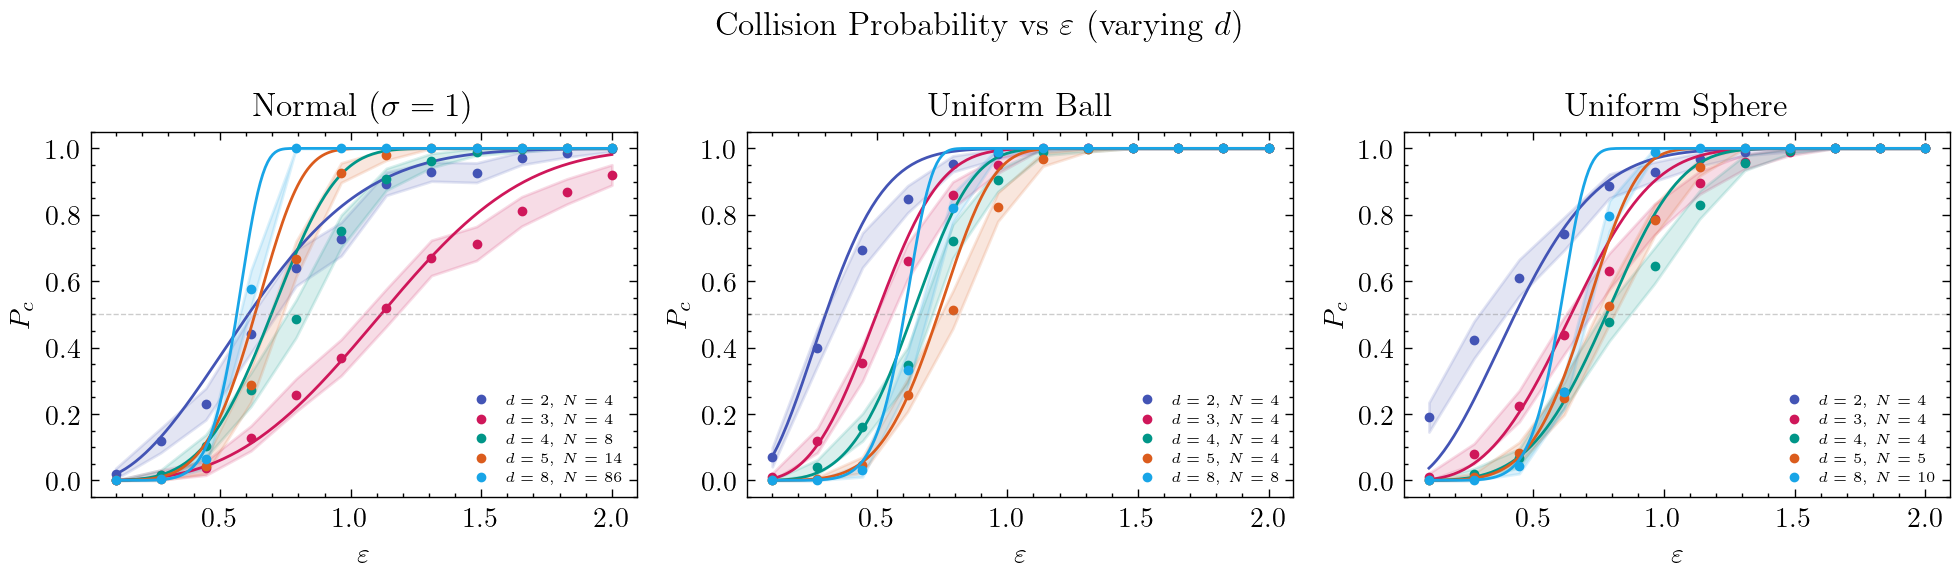
\includegraphics[width=\linewidth]{plots/Pc_vs_eps.png}
    \caption{Collision probability as a function of $\varepsilon$ at fixed $N$ near the predicted capacity. Theory and simulation converge as dimension grows.}
    \label{fig:Pc_vs_eps}
\end{figure}

\begin{figure}[t]
    \centering
    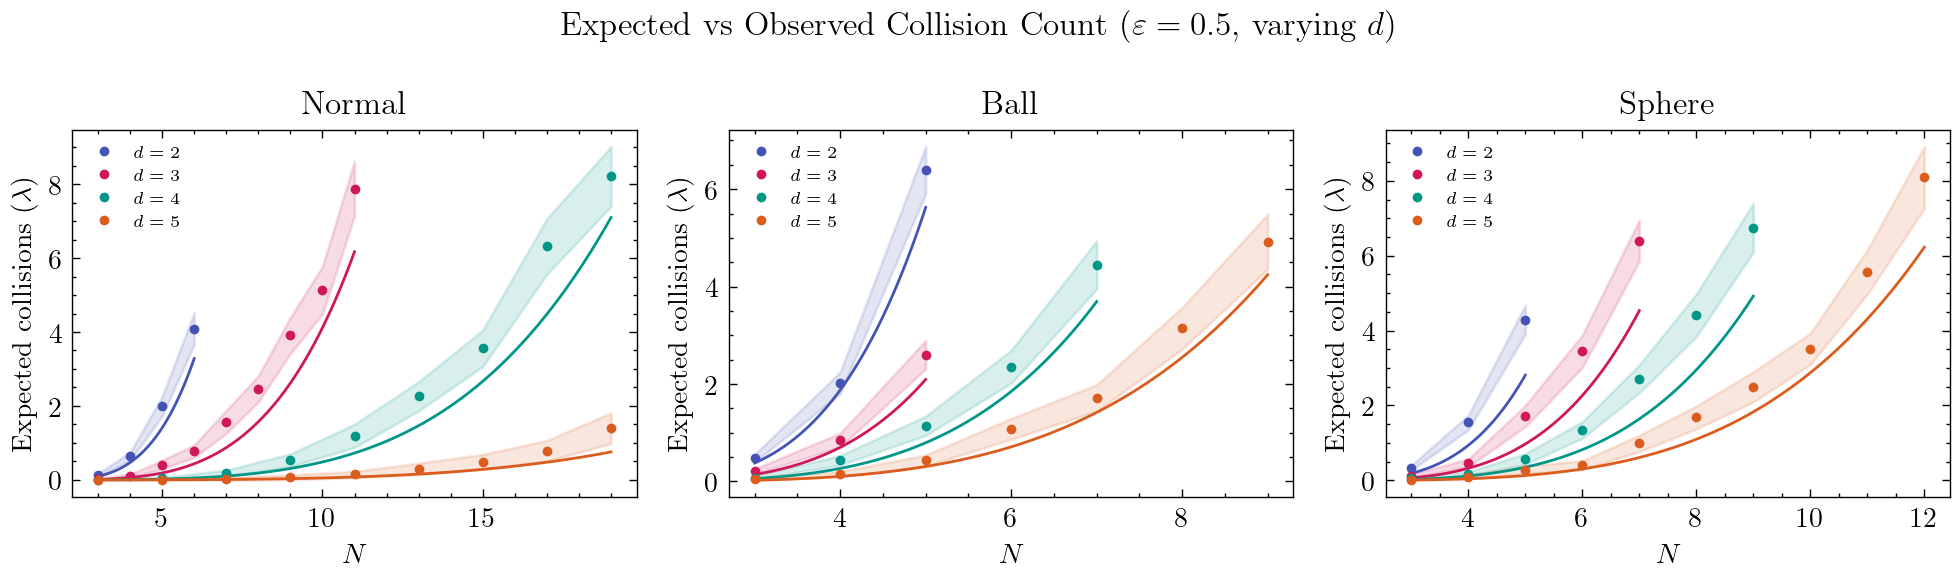
\includegraphics[width=\linewidth]{plots/lambda_vs_collisions.png}
    \caption{Poisson mean $\lambda$ vs.\ observed mean collision count. The approximation is accurate for $d \ge 3$.}
    \label{fig:lambda}
\end{figure}

\begin{figure}[t]
    \centering
    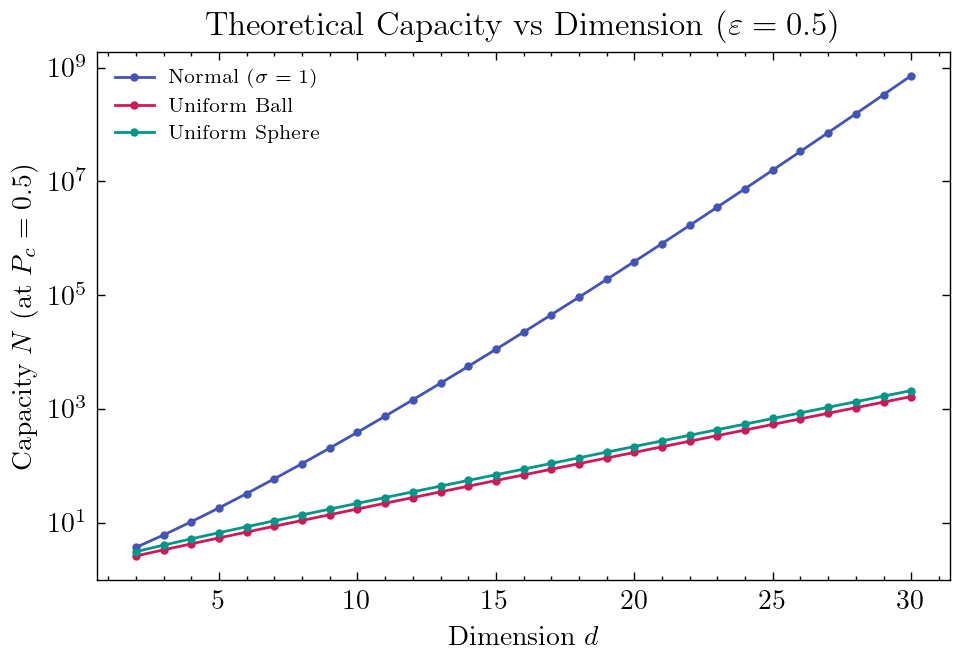
\includegraphics[width=0.55\linewidth]{plots/capacity_vs_d.png}
    \caption{Theoretical capacity $N^\star$ vs.\ dimension at $\varepsilon = 0.5$. Gaussian capacity grows exponentially faster than compactly supported distributions.}
    \label{fig:cap_vs_d}
\end{figure}

\begin{figure}[t]
    \centering
    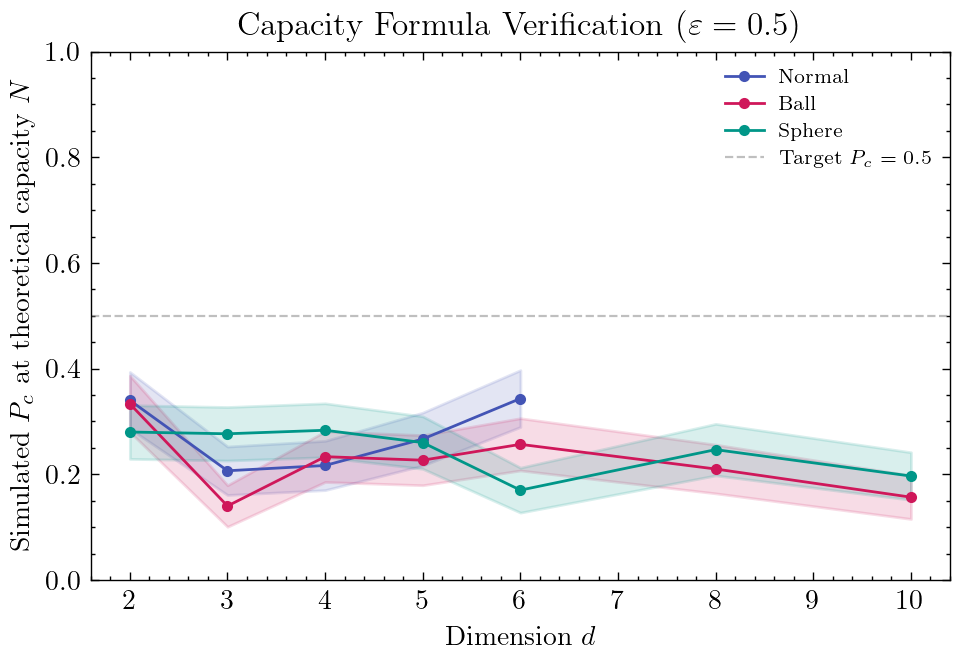
\includegraphics[width=0.55\linewidth]{plots/capacity_verification.png}
    \caption{Simulated $P_c$ at the theoretical $N^\star$. Values lie below $1/2$, confirming \eqref{eq:capacity} as a conservative lower bound.}
    \label{fig:cap_verify}
\end{figure}

\FloatBarrier

% ==============================================================
\section{Discussion}
\label{sec:discussion}

\paragraph{Separating flatness from isotropy.} The geometric argument of \secref{sec:geometry} decomposes into two independent claims. Flatness ($\R^d$, no normalization) is necessary and sufficient for Euclidean differencing to satisfy the change vector axioms and for semantic consistency to hold in the compact-cluster limit. Isotropy ($\mathrm{Cov} \approx \mat{I}$) is a separate property that ensures change magnitudes are calibrated and direction-independent. A flat but highly anisotropic space would have well-defined change vectors whose magnitudes are difficult to interpret; a curved but isotropic space (the standard sphere) has calibrated distances but ill-defined differences. Both properties are needed, but for different reasons.

\paragraph{Conservatism of the capacity bound.} The $N^4/8$ pair count overcounts by including candidate pairs of differences that share an endpoint. These are not independent collision events, so \eqref{eq:capacity} is a lower bound on true capacity (\figref{fig:cap_verify}). The CLT approximation for $f_{\vect{Z}}(\vect{0})$ also degrades at small $d$ but is nearly exact in the regime ($d \gtrsim 64$) where change detection is deployed. The conservative character is an asset: the formula guarantees that collision probability is at most $1/2$, and in practice it is strictly lower.

\paragraph{Practical implications.} For typical deployment parameters ($d \ge 128$, $\varepsilon \sim 0.5$, $\sigma \sim 1$) the Gaussian capacity is astronomical, so collisions are not a binding constraint for any realistic dataset. The formulas matter as a structural characterization: they make explicit the tradeoff between embedding dimensionality ($d$), collision tolerance ($\varepsilon$), and spatial spread ($\sigma$).

\paragraph{Limitations.} This work is purely theoretical---we do not train encoders or evaluate downstream change detection. The semantic consistency definition assumes discrete classes; extending it to continuous or hierarchical structures is future work. The capacity analysis assumes i.i.d.\ embeddings, an idealization for learned representations.


% ==============================================================
\section*{Summary}

Embedding differencing for change detection requires a flat geometry. On the hypersphere, any change-vector operator incurs a curvature-driven error that grows with how far apart the points are (Proposition~\ref{prop:composability_floor}), ambient differencing is semantically inconsistent (Proposition~\ref{prop:ambient_bad}), and concatenation abandons geometric structure entirely. A flat embedding space resolves the first two failures (Proposition~\ref{prop:flat_sufficient}); regularizing toward an isotropic Gaussian further calibrates change magnitudes (Proposition~\ref{prop:isotropy_calibration}). Together, these make Euclidean subtraction a composable, semantically consistent, and calibrated change operator. In such a space, the expected capacity scales as $N^\star \propto (\sigma/\varepsilon)^{d/4}$, verified empirically, and is not a binding constraint for practical dimensionalities.

\FloatBarrier
\bibliographystyle{plainnat}
\bibliography{references}

\end{document}